\documentclass[a4paper,12pt]{article}
\usepackage[french]{babel}
\usepackage[utf8]{inputenc}
\usepackage[T1]{fontenc}
\usepackage{graphicx}
\usepackage{geometry}
\usepackage{fancyhdr}
\usepackage{hyperref}
\usepackage{titlesec}
\usepackage{xcolor}
\usepackage{listings}
\usepackage{enumitem}
\usepackage{eso-pic}
\usepackage{tikz}
\usepackage{array}
\usepackage{tcolorbox}
\usepackage{fancyvrb}
\usepackage{needspace}
\usepackage{caption}
\usepackage{placeins}
\usepackage{float}

\geometry{left=2.5cm,right=2.5cm,top=2.5cm,bottom=2.5cm}
\setlength{\headheight}{14.5pt}

\pagestyle{fancy}
\fancyhf{}
\rhead{\thepage}
\lhead{Projet Linux AWS}
\renewcommand{\headrulewidth}{0.4pt}

\definecolor{background}{RGB}{250,250,252}
\definecolor{string}{RGB}{170,85,102}
\definecolor{comment}{RGB}{120,120,125}
\definecolor{keyword}{RGB}{70,130,180}
\definecolor{identifier}{RGB}{85,140,85}
\definecolor{frame}{RGB}{230,230,235}
\definecolor{linenumber}{RGB}{160,160,165}

\lstset{
    basicstyle=\ttfamily\footnotesize,
    backgroundcolor=\color{background},
    frame=single,
    rulecolor=\color{frame},
    framexleftmargin=8pt,
    framexrightmargin=8pt,
    framextopmargin=6pt,
    framexbottommargin=6pt,
    framesep=6pt,
    breaklines=true,
    breakatwhitespace=true,
    showstringspaces=false,
    keywordstyle=\color{keyword}\bfseries,
    stringstyle=\color{string},
    commentstyle=\color{comment}\itshape,
    identifierstyle=\color{identifier},
    captionpos=b,
    numbers=none,
    xleftmargin=20pt,
    xrightmargin=20pt,
    aboveskip=15pt,
    belowskip=15pt,
    lineskip=1pt,
    columns=flexible,
    keepspaces=true,
    tabsize=4,
    showspaces=false,
    showtabs=false,
    prebreak=\raisebox{0ex}[0ex][0ex]{\ensuremath{\hookleftarrow}},
    postbreak=\raisebox{0ex}[0ex][0ex]{\ensuremath{\hookrightarrow\space}},
    breakindent=1.5em,
    float=htbp,
    floatplacement=H
}

\titleformat{\section}{\large\bfseries}{\thesection}{1em}{}
\titleformat{\subsection}{\normalsize\bfseries}{\thesubsection}{1em}{}

\renewcommand{\lstlistingname}{Configuration}
\renewcommand{\lstlistlistingname}{Table des configurations}

\AddToShipoutPictureBG{%
  \begin{tikzpicture}[remember picture, overlay]
    \node[anchor=south east, xshift=-2.5cm, yshift=1cm] at (current page.south east)
      {
\includegraphics[width=0.3\textwidth]{/home/samet/Documents/projet-linux-aws/documentations/report/fwb.png}};
    \node[anchor=south west, xshift=2.5cm, yshift=0.75cm] at (current page.south west)
      {
\includegraphics[width=0.2\textwidth]{/home/samet/Documents/projet-linux-aws/documentations/report/logo.png}};
    \node[anchor=south west, xshift=1cm, yshift=1cm] at (current page.south west)
      {
\includegraphics[width=0.02\textwidth]{/home/samet/Documents/projet-linux-aws/documentations/report/side.png}};
  \end{tikzpicture}%
}

\makeatletter
  \setlength{\@fptop}{0pt}
  \setlength{\@fpsep}{5pt plus 1pt minus 1pt}
  \setlength{\@fpbot}{0pt}
\makeatother

\setlength{\intextsep}{5pt plus 1pt minus 1pt}

\begin{document}

\begin{titlepage}
	\begin{tikzpicture}[remember picture, overlay]
		\node[anchor=north west, inner sep=0pt] at (current page.north west)
		{
\includegraphics[width=\paperwidth]{/home/samet/Documents/projet-linux-aws/documentations/report/entete.png}};
	\end{tikzpicture}
	
	\vspace*{7cm}
	\centering
	{\Huge\textbf{Projet Linux AWS}\par}
	\vspace{0.5cm}
	{\LARGE Rapport Final\par}
	\vfill
	\flushright
	\textbf{Année Académique\\}2024 - 2025 \\[0.5cm]
	\textbf{Auteurs}\\Adam Bougma\\Samet Catakli\\
\end{titlepage}

\tableofcontents
\newpage

\lstlistoflistings
\newpage

\listoffigures
\newpage

\section{Introduction}

Dans le cadre du projet Linux AWS, nous avons mis en place une infrastructure sécurisée et complète afin de proposer un service d'hébergement web multi-utilisateur. Ce rapport technique présente les choix technologiques, les configurations effectuées ainsi que les mesures de sécurité mises en oeuvre pour assurer un service fiable et sécurisé.

\section{Plan de l'infrastructure}

\subsection{Architecture initiale prévue}

Notre conception initiale prévoyait une infrastructure modulaire composée de plusieurs serveurs spécialisés :

\begin{itemize}
    \item \textbf{Serveur Réseau} : Dédié aux services DNS (BIND9) et synchronisation temporelle (NTP), assurant ainsi les fonctions fondamentales d'infrastructure.
    \item \textbf{Serveur Web} : Hébergeant Apache, PHP, MariaDB et les services de partage de fichiers (Samba, FTP, NFS).
    \item \textbf{Serveur de Monitoring} : Dédié à la surveillance de l'infrastructure via Netdata.
    \item \textbf{Solution de Sauvegarde} : Initialement prévue sur AWS S3/Glacier pour stocker les sauvegardes de manière économique et durable.
\end{itemize}

\subsection{Architecture effective déployée}

En raison des contraintes de temps et des difficultés rencontrées avec l'API AWS pour accéder à S3, nous avons adapté notre infrastructure :

\begin{itemize}
    \item \textbf{Instance principale} (10.42.0.109) : Regroupant les services réseau (DNS, NTP) et les services web (Apache, PHP, MariaDB, partage de fichiers).
    \item \textbf{Instance secondaire} (10.42.0.129) : Combinant les fonctions de monitoring (Netdata) et servant de destination pour les sauvegardes via SCP.
\end{itemize}

Les deux instances sont déployées dans un VPC (Virtual Private Cloud) sur le réseau 10.42.0.0/24, accéssible uniquement via vpn,  offrant une isolation réseau et une communication sécurisée entre les composants de l'infrastructure.

Cette architecture simplifiée nous a permis de fournir tous les services requis tout en contournant les problèmes d'accès à S3, offrant une solution robuste qui respecte les exigences du projet.

\section{Choix technologiques}

\subsection{Distribution Linux}

Dans le cadre de ce projet, la distribution imposée était \texttt{Amazon Linux 2023} (al2023), développée par Amazon pour une intégration optimale avec l'infrastructure AWS. Elle repose sur un noyau léger, sécurisé et optimisé pour l'environnement AWS, offrant ainsi des performances élevées tout en garantissant un haut niveau de sécurité. Par ailleurs, cette distribution est volontairement minimaliste : très peu de paquets sont installés par défaut, ce qui permet de limiter la surface d'attaque en réduisant l'exposition à d'éventuelles vulnérabilités liées à des services non nécessaires. Basée sur RHEL, elle supporte aussi nativement SELINUX, qui est un module critique pour la sécurité renforcée.

\subsection{Méthode d'installation}

Le déploiement des instances a été réalisé de manière automatisée via la console AWS, permettant une mise en service rapide et standardisée. Une phase de configuration manuelle complémentaire a ensuite été effectuée, soit par accès SSH depuis un terminal, soit directement via l'interface de la console AWS, afin d'adapter finement les paramètres système et de sécurité aux besoins spécifiques du projet.

\section{Plan de partitionnement}

Les technologies LVM et RAID ont été utilisées pour la gestion des disques et le partitionnement. Bien qu'un RAID5 soit mis en place par défaut sur AWS, nous avons configuré un RAID1  avec les disques \texttt{/dev/nvme1n1} et \texttt{/dev/nvme2n1} attachés à l'instance et montés sur \texttt{/srv}. Un partitionnement LVM a été configuré sur ce RAID pour bénéficier des fonctionnalités de gestion avancées, telles que les snapshots et le redimensionnement à chaud.

Le partitionnement choisi permet d'optimiser sécurité, performance et gestion des données :

\begin{itemize}
	\item \textbf{/} : système d'exploitation, configurations globales.
	\item \textbf{/boot} : fichiers de démarrage, noyaux Linux.
	\item \textbf{/tmp} : pour les fichiers temporaires.
	\item \textbf{/etc} : configurations spécifiques des services.
	\item \textbf{/var} : fichiers dynamiques tels que logs système et fichiers temporaires d'applications.
	\item \textbf{/home} : espaces utilisateurs. (très peu utilisé dans notre système)
	\item \textbf{/srv} : structuré spécifiquement en RAID1 et LVM, contenant :
	\begin{itemize}
		\item \texttt{/srv/web} : fichiers des sites web hébergés (avec partage ftp/samba privé) .
		\item \texttt{/srv/database} : stockage des bases de données (mariadb datadir).
		\item \texttt{/srv/share} : données partagées non privé(NFS, Samba, FTP).
	\end{itemize}
\end{itemize}

\clearpage
\section{Description des services déployés}

\subsection{Services réseau}

\paragraph{Serveur DNS (BIND9)}

Le serveur DNS a été mis en place à l'aide de BIND9, en s'appuyant sur le service named pour assurer la résolution des noms de domaine. Il prend en charge à la fois la résolution directe (DNS) et inverse (reverse DNS), ce qui permet d'héberger une zone DNS locale ainsi que les enregistrements associés aux noms de domaine utilisés par les clients du réseau. Pour garantir l'accès aux domaines externes — notamment pour les mises à jour logicielles ou les accès internet — un mécanisme de forwarding a été configuré : les requêtes en dehors de la zone locale sont redirigées vers les serveurs DNS publics de Cloudflare. Cette approche assure à la fois une résolution rapide, fiable et sécurisée des noms externes, tout en gardant un contrôle total sur la zone DNS interne.

\needspace{8\baselineskip}
\begin{lstlisting}[caption={Configuration DNS BIND9 – /etc/named.conf}]
options {
    listen-on port 53 { any; };
    directory "/var/named";
    recursion yes;
    allow-query { any; };
    allow-transfer { none; };
    dnssec-validation auto;
};

zone "." IN {
    type hint;
    file "named.ca";
};

zone "heh.cloud" IN {
    type master;
    file "forward.heh.cloud";
    allow-update { none; };
};

zone "0.42.10.in-addr.arpa" IN {
    type master;
    file "reverse.heh.cloud";
    allow-update { none; };
};
\end{lstlisting}

\needspace{6\baselineskip}
\begin{lstlisting}[caption={Configuration DNS BIND9 – /var/named/forward.heh.cloud}]
$TTL 86400
@   IN  SOA     ns.heh.cloud. root.heh.cloud. (
            2024052101 ; Serial
            3600       ; Refresh
            1800       ; Retry
            604800     ; Expire
            86400 )    ; Minimum TTL

@       IN  NS      ns.heh.cloud.
ns      IN  A       10.42.0.109
@       IN  A       10.42.0.109
*       IN  A       10.42.0.109
\end{lstlisting}

Des mesures de sécurité spécifiques ont été appliquées :
\begin{itemize}
    \item Limitation des transferts de zone (\texttt{allow-transfer \{ none; \}})
    \item Configuration du service pour écouter uniquement sur les interfaces nécessaires
    \item Utilisation de \texttt{dnssec-validation auto} pour renforcer la sécurité des réponses DNS
\end{itemize}

\paragraph{Serveur NTP (Chrony)}

Chrony a été configuré pour assurer une synchronisation précise de l'horloge système sur le fuseau horaire \texttt{Europe/Bruxelles}. Dans cette infrastructure, un serveur NTP interne a été mis en place pour servir de référence temporelle principale. Les autres machines du réseau sont configurées pour se synchroniser avec ce serveur, ce qui garantit une cohérence horaire uniforme à l'échelle de l'ensemble du système. Ce choix permet non seulement de limiter la dépendance à des serveurs externes, mais aussi de réduire la latence et d'améliorer la sécurité des échanges temporels au sein du réseau local.

\needspace{6\baselineskip}
\begin{lstlisting}[caption={Configuration NTP Chrony – /etc/chrony.conf}]
# Server directives specify NTP servers to use
server 0.pool.ntp.org iburst
server 1.pool.ntp.org iburst
server 2.pool.ntp.org iburst
server 3.pool.ntp.org iburst

# Allow NTP client access from local network
allow 10.42.0.0/24

# Record the rate at which the system clock gains/losses time
driftfile /var/lib/chrony/drift
\end{lstlisting}

\subsection{Partage de fichiers}

\paragraph{Samba}

Samba a été mis en place pour offrir un service de partage de fichiers sécurisé entre systèmes Windows et Linux. Dans la configuration, on trouve à la fois des répertoires publics, accessibles à tous les utilisateurs, et des répertoires privés, protégés par des droits d'accès individuels. Des comptes Samba spécifiques, associés à des utilisateurs du système, assurent une gestion fine des permissions, ce qui permet un contrôle complet des lectures, écritures et modifications des fichiers partagés.

\needspace{8\baselineskip}
\begin{lstlisting}[caption={Configuration Samba – /etc/samba/smb.unauth.conf}]
[unauth_share]
   path = /srv/share/
   browsable = yes
   writable = yes
   guest ok = yes
   guest only = yes
   force user = nobody
   force group = nobody
   create mask = 0777
   directory mask = 0777
   read only = no
\end{lstlisting}

\needspace{6\baselineskip}
\begin{lstlisting}[caption={Configuration Samba – /etc/samba/smb.conf}]
[global]
    workgroup = SAMBA
    security = user
    passdb backend = tdbsam
    include = /etc/samba/usershares.conf
        
[username]
    path = /srv/web/username
    valid users = username
    read only = no
\end{lstlisting}

\paragraph{FTP}

Pour garantir des transferts de fichiers sécurisés, le serveur FTP a été configuré en utilisant le chiffrement TLS (FTPS). Ce chiffrement assure la confidentialité et l'intégrité des données échangées entre le client et le serveur, en protégeant les identifiants et les fichiers contre toute interception. Les ressources sont accessibles uniquement aux utilisateurs authentifiés, et les droits d'accès sont strictement définis pour chaque utilisateur lié aux comptes système. Cette solution garantit la compatibilité avec les clients FTP traditionnels tout en répondant aux exigences de sécurité actuelles.

\needspace{10\baselineskip}
\begin{lstlisting}[caption={Configuration FTP vsftpd – /etc/vsftpd/vsftpd.conf}]
anonymous_enable=YES
local_enable=YES
write_enable=YES
anon_upload_enable=YES
anon_mkdir_write_enable=YES

dirmessage_enable=YES
xferlog_enable=YES
connect_from_port_20=YES
xferlog_std_format=YES
listen=YES
listen_ipv6=NO

pam_service_name=vsftpd
userlist_enable=YES
anon_root=/srv/share/ftp
anon_umask=022

pasv_enable=YES
pasv_min_port=30000
pasv_max_port=31000
\end{lstlisting}

\paragraph{NFS (public uniquement)}

NFS, un système de partage de fichiers disponible uniquement sur Linux, est utilisé uniquement pour le partage public de fichiers. Disposant uniquement de contrôle d'accès basé sur les adresses IP (ACL), il ne convient pas aux partages privés nécessitant une authentification. Il est donc limité dans ce projet aux répertoires accessibles à tous les utilisateurs du réseau local.

\needspace{3\baselineskip}
\begin{lstlisting}[caption={Configuration NFS – /etc/exports}]
/srv/share *(rw,sync,no_root_squash)
\end{lstlisting}

\clearpage
\subsection{Serveur web (Apache et PHP)}

Le serveur web Apache a été choisi pour sa popularité, sa robustesse et sa flexibilité (modules). Couplée au langage PHP, elle permet d'héberger des sites dynamiques avec code backend.

\needspace{10\baselineskip}
\begin{lstlisting}[caption={Configuration Apache – /etc/httpd/conf.d/heh.cloud.conf}]
<VirtualHost *:80>
    ServerName heh.cloud
    ServerAlias *.heh.cloud
    DocumentRoot /srv/web/root
    <Directory /srv/web/root>
        AllowOverride All
        Require all granted
    </Directory>
    DirectoryIndex index.php
    
    # Journalisation
    ErrorLog /var/log/httpd/root_error.log
    CustomLog /var/log/httpd/root_access.log combined

    # Redirection vers HTTPS
    Redirect "/" "https://heh.cloud/"
</VirtualHost>
\end{lstlisting}

\needspace{12\baselineskip}
\begin{lstlisting}[caption={Configuration Apache SSL – /etc/httpd/conf.d/heh.cloud-ssl.conf}]
<VirtualHost *:443>
    ServerName heh.cloud
    ServerAlias *.heh.cloud
    DocumentRoot /srv/web/root
    
    <Directory /srv/web/root>
        AllowOverride All
        Require all granted
    </Directory>
    
    DirectoryIndex index.php
    
    # Configuration SSL
    SSLEngine on
    SSLCertificateFile /etc/httpd/ssl/heh.cloud.crt
    SSLCertificateKeyFile /etc/httpd/ssl/heh.cloud.key
    
    # Journalisation
    ErrorLog /var/log/httpd/root_ssl_error.log
    CustomLog /var/log/httpd/root_ssl_access.log combined
</VirtualHost>
\end{lstlisting}

MariaDB, un fork de MySQL offrant davantage de fonctionnalités et une meilleure performance dans certains cas, a été choisie comme système de gestion de base de données. Elle a été configurée pour stocker ses fichiers de données sur la partition en RAID 1/LVM \texttt{/srv/database}, garantissant ainsi une redondance et une meilleure tolérance aux pannes.

\needspace{4\baselineskip}
\begin{lstlisting}[caption={Configuration MariaDB – /etc/my.cnf.d/server.cnf}]
[mysqld]
datadir=/srv/database
socket=/var/lib/mysql/mysql.sock

[client]
socket=/var/lib/mysql/mysql.sock
\end{lstlisting}

Phpmyadmin, une application web qui permet une gestion simplifiée des bases de données, a été choisie et mise à la disposition des utilisateurs pour gérer leurs bases de données. Les paramètres suivants ont été mis en place :

\needspace{15\baselineskip}
\begin{lstlisting}[caption={Configuration phpMyAdmin – /etc/httpd/conf.d/phpmyadmin.conf}]
<VirtualHost *:443>
    ServerName phpmyadmin.heh.cloud
    DocumentRoot /srv/web/phpmyadmin

    <Directory /srv/web/phpmyadmin/>
        AddDefaultCharset UTF-8
        Options FollowSymLinks
        AllowOverride All
        Require all granted

        # Block root user access
        <IfModule mod_rewrite.c>
            RewriteEngine On
            RewriteCond %{REQUEST_URI} ^/.*
            RewriteCond %{REQUEST_METHOD} ^POST$
            RewriteCond %{REQUEST_URI} !server-status
            RewriteCond %{THE_REQUEST} pma_username=root [NC]
            RewriteRule .* - [F,L]
        </IfModule>
    </Directory>

    <Directory /srv/web/phpmyadmin/libraries/>
        Require all denied
    </Directory>

    SSLEngine on
    SSLCertificateFile /etc/httpd/ssl/heh.cloud.crt
    SSLCertificateKeyFile /etc/httpd/ssl/heh.cloud.key
</VirtualHost>
\end{lstlisting}

\needspace{10\baselineskip}
\begin{lstlisting}[caption={Configuration phpMyAdmin – /srv/web/phpmyadmin/config.inc.php}]
<?php
// Secret key pour l'authentification par cookie
$cfg['blowfish_secret'] = 'BLOWFISH_SECRET';

$i = 0;
$i++;
$cfg['Servers'][$i]['auth_type'] = 'cookie';
$cfg['Servers'][$i]['host'] = 'localhost';
$cfg['Servers'][$i]['socket'] = '/var/lib/mysql/mysql.sock';
$cfg['Servers'][$i]['compress'] = false;
$cfg['Servers'][$i]['AllowNoPassword'] = false;
$cfg['Servers'][$i]['AllowRoot'] = false; // Désactivation de l'accès root

$cfg['UploadDir'] = '';
$cfg['SaveDir'] = '';
$cfg['SendErrorReports'] = 'never';
?>
\end{lstlisting}

\subsection{Monitoring}

L'application  \texttt{Netdata} est utilisée pour surveiller en temps réel les performances et l'état de santé du système ainsi que des différents services. Elle permet notamment de surveiller les ressources du serveur, le trafic réseau et http, et l'état de santé des différents services configurés tels que le serveur web, Samba, MariaDB, DNS, etc. Un dashboard personnalisé et des alertes ont été configurés pour une meilleure prise en main et des interventions rapides.

\begin{figure}[htbp]
    \centering
    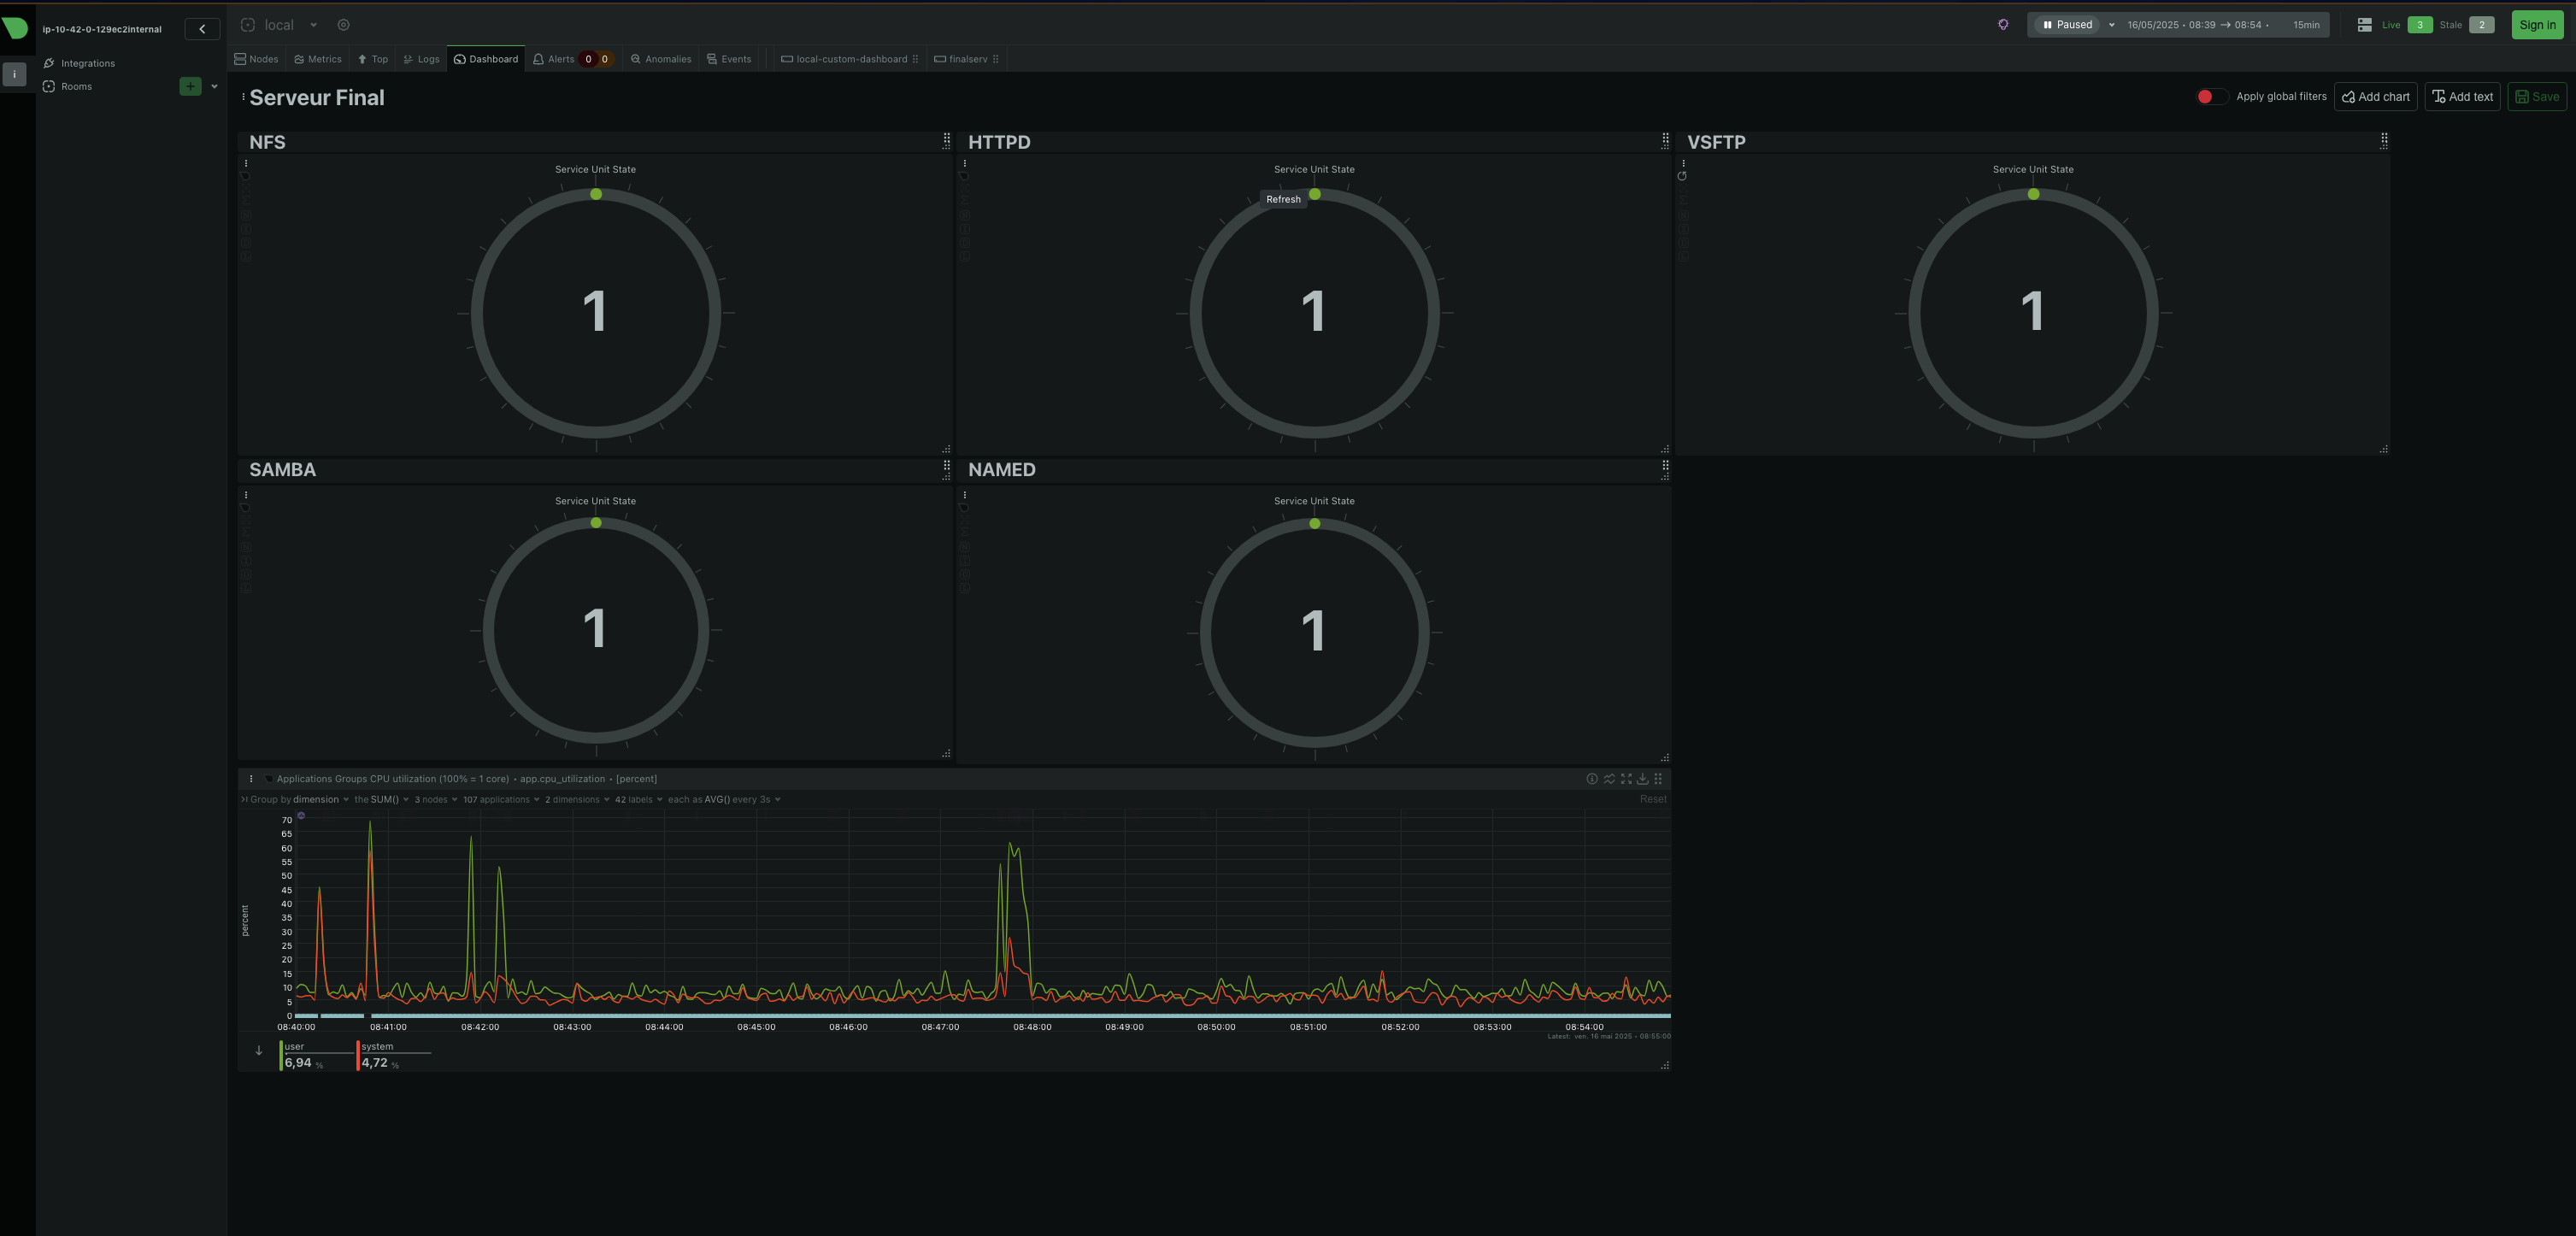
\includegraphics[width=\textwidth]{netdata.png}
    \caption{Dashboard Netdata montrant l'état de santé du système et des services.}
    \label{fig:netdata-dashboard}
\end{figure}

\needspace{6\baselineskip}
\begin{lstlisting}[caption={Configuration Netdata Serveur – /etc/netdata/stream.conf}]
[stream]
  enabled = yes
  api key = API_KEY
  default memory mode = ram
  health enabled by default = auto
  allow from = *
\end{lstlisting}

\needspace{4\baselineskip}
\begin{lstlisting}[caption={Configuration Netdata Client – /etc/netdata/stream.conf}]
[stream]
  enabled = yes
  destination = 10.42.0.129:19999
  api key = API_KEY
\end{lstlisting}

\section{Plan de sauvegarde}

Un plan de sauvegarde robuste vers S3 Glacier avait initialement été conçu pour effectuer des sauvegardes économiques vers un bucket AWS. Une sauvegarde incrémentielle quotidienne et une complète hebdomadaire avaient été pensées. Cependant, en raison de problèmes d'accès avec les clés API refusées, nous avons opté pour une solution alternative avec des sauvegardes envoyées vers la partition RAID/LVM  \texttt{/srv/backup} de l'instance secondaire sur laquelle se trouve l'application de monitoring.\\\\
Voici une liste des partitions sauvegardées:
\begin{itemize}
	\item \textbf{/etc} : configurations spécifiques des services.
	\item \textbf{/var} : fichiers dynamiques tels que logs système.
	\item \textbf{/home} : espaces utilisateurs. (très peu utilisé dans notre système)
	\item \texttt{/srv/web} : fichiers des sites web hébergés.
	\item \texttt{/srv/database} : fichiers de base de données.
	\item \texttt{/srv/share} : données partagées non privé (NFS, Samba, FTP).
\end{itemize}

\needspace{3\baselineskip}
\begin{lstlisting}[caption={Configuration Sauvegarde – /etc/crontab}]
0 2 * * * /path/to/backup.sh >> /var/log/backup.log 2>&1
\end{lstlisting}

Cette tâche cron exécute quotidiennement à 2h du matin un script de sauvegarde qui transfère les données critiques vers l'instance de backup via rsync et SSH.

\clearpage
\section{Sécurité avancée du serveur}

\subsection{Configuration SSH}

Afin de garantir un accès sécurisé au serveur, une configuration SSH renforcée a été mise en œuvre. La connexion directe en tant qu'utilisateur root a été désactivée, tout comme l'authentification par mot de passe, afin de réduire les risques liés aux attaques par force brute ou à l'utilisation de mots de passe faibles. Seules les connexions via des paires de clés SSH sont autorisées, assurant ainsi une méthode d'authentification plus robuste. De plus, l'activation des journaux de connexion permet un suivi précis des accès, tandis que l'intégration de Fail2Ban contribue à bloquer automatiquement les tentatives suspectes, ajoutant une couche supplémentaire de protection à l'interface SSH.

\needspace{6\baselineskip}
\begin{lstlisting}[caption={Configuration SSH – /etc/ssh/sshd\textunderscore config}]
# Authentification par clé uniquement
PasswordAuthentication no

# Blocage de l'accès root
PermitRootLogin no

# Journalisation avancée
LogLevel VERBOSE

# Autres options de sécurité
PubkeyAuthentication yes
Protocol 2
X11Forwarding no
\end{lstlisting}

\subsection{Firewalls}

Deux niveaux de protection par pare-feu ont été déployés afin de sécuriser les communications réseau tout en optimisant les performances du système. Les  \texttt{Security Groups} d'AWS agissent comme un pare-feu périmétrique en filtrant le trafic au niveau de l'infrastructure cloud, ce qui permet de bloquer les connexions non autorisées avant même qu'elles n'atteignent l'instance. Ce filtrage en amont contribue à éviter une surcharge inutile des ressources du serveur, en empêchant le traitement de requêtes malveillantes ou superflues. En complément,  \texttt{firewalld} est utilisé au niveau de l'instance pour affiner la politique de sécurité interne, assurant un contrôle granulaire des flux autorisés selon les services et les zones définies. Cette approche à deux niveaux renforce à la fois la sécurité et l'efficacité de la gestion du trafic réseau.

\needspace{12\baselineskip}
\begin{lstlisting}[caption={Configuration Firewalld – Commandes de configuration}]
# Configuration des zones
firewall-cmd --set-default-zone=public

# Services autorisés
firewall-cmd --permanent --zone=public --add-service=ssh
firewall-cmd --permanent --zone=public --add-service=http
firewall-cmd --permanent --zone=public --add-service=https
firewall-cmd --permanent --zone=public --add-service=dns
firewall-cmd --permanent --zone=public --add-service=ftp
firewall-cmd --permanent --zone=public --add-service=mysql
firewall-cmd --permanent --zone=public --add-service=samba
firewall-cmd --permanent --zone=public --add-service=nfs

# Ports spécifiques
firewall-cmd --permanent --zone=public --add-port=19999/tcp  # Netdata
firewall-cmd --permanent --zone=public --add-port=30000-31000/tcp  # FTP passif
\end{lstlisting}

\subsection{SELinux}

SELinux (Security-Enhanced Linux), un module de sécurité développé par la NSA pour fournir un contrôle d'accès renforcé, a été activé en mode \texttt{enforcing}, ce qui signifie que toutes les politiques de sécurité sont strictement appliquées. Des règles strictes ont été mises en place, afin de n'autoriser que les actions strictement nécessaires au bon fonctionnement du système. Cette approche permet de limiter les risques liés aux attaques et d'atteindre une sécurité de niveau entreprise.

\needspace{10\baselineskip}
\begin{lstlisting}[caption={Configuration SELinux – /etc/selinux/config}]
# Activation de SELinux en mode enforcing
setenforce 1
sed -i 's/^SELINUX=.*/SELINUX=enforcing/' /etc/selinux/config

# Configuration des  booleans SELinux
setsebool -P httpd_can_network_connect_db 1
setsebool -P httpd_can_network_connect 1
setsebool -P samba_export_all_rw 1
setsebool -P ftpd_full_access 1
setsebool -P ssh_sysadm_login 1

# Configuration du contexte pour les répertoires web
semanage fcontext -a -t httpd_sys_content_t "/srv/web(/.*)?"
restorecon -Rv /srv/web
\end{lstlisting}

\needspace{5\baselineskip}
\begin{lstlisting}[caption={Configuration SELinux – Politique PHP-FPM - MySQL}]
#  Pour autoriser PHP-FPM à se connecter au socket MySQL
module php_mysql_fix 1.0;

allow httpd_t mysqld_t:unix_stream_socket connectto;
allow httpd_t mysqld_var_run_t:sock_file write;
\end{lstlisting}

\subsection{Options de montage sécurisées}

Des options de montage spécifiques ont été définies dans le fichier  \texttt{/etc/fstab} afin de renforcer la sécurité des différentes partitions du système. Ces options permettent, par exemple, d'empêcher l'exécution de fichiers binaires ( \texttt{noexec}), l'écriture sur certaines partitions ( \texttt{ro, nosuid, nodev}), ou encore de limiter les privilèges d'accès. Ce type de configuration réduit la surface d'attaque en restreignant les comportements potentiellement dangereux sur certaines zones du système de fichiers.

\needspace{8\baselineskip}
\begin{lstlisting}[caption={Configuration Système – /etc/fstab}]
# Montage en lecture seule du bootloader
/dev/nvme0n1p1 /boot/efi vfat umask=0077,ro 0 2

# Protection du répertoire temporaire
tmpfs /tmp tmpfs defaults,noexec,nosuid,nodev,size=2G 0 0

# Protection des répertoires utilisateurs
/dev/mapper/vg-home /home xfs defaults,nodev 0 2

# Protection des partages
/dev/mapper/vg_raid-share /srv/share ext4 defaults,usrquota,grpquota,nodev 0 2
/dev/mapper/vg_raid-web /srv/web ext4 defaults,usrquota,grpquota,nodev 0 2
\end{lstlisting}

\subsection{Fail2Ban}

Fail2Ban est un outil de sécurité permettant de protéger le système contre les attaques par force brute en surveillant les fichiers journaux de plusieurs services critiques (comme SSH, FTP, SMTP, Apache, etc.). Lorsqu'il détecte des tentatives de connexion répétées échouées, il bloque automatiquement l'adresse IP de l'attaquant en configurant temporairement le pare-feu, réduisant ainsi les risques d'intrusion ou d'exploitation.\\
Voici les configuration fail2ban déploiyé: 

\needspace{5\baselineskip}
\begin{lstlisting}[caption={Configuration Fail2Ban SSH – /etc/fail2ban/jail.d/sshd.local}]
[sshd]
enabled = true
port = ssh
filter = sshd
logpath = /var/log/secure
maxretry = 10
bantime = 3600
\end{lstlisting}

\needspace{5\baselineskip}
\begin{lstlisting}[caption={Configuration Fail2Ban FTP – /etc/fail2ban/jail.d/ftp.local}]
[vsftpd]
enabled = true
port = ftp,ftp-data,ftps,ftps-data
filter = vsftpd
logpath = /var/log/secure
maxretry = 3
bantime = 3600
\end{lstlisting}

\needspace{5\baselineskip}
\begin{lstlisting}[caption={Configuration Fail2Ban Apache – /etc/fail2ban/jail.d/apache.local}]
[apache-auth]
enabled = true
port = http,https
filter = apache-auth
logpath = /var/log/httpd/*error_log
maxretry = 3
bantime = 3600
\end{lstlisting}

\needspace{5\baselineskip}
\begin{lstlisting}[caption={Configuration Fail2Ban Samba – /etc/fail2ban/jail.d/samba.local}]
[samba]
enabled = true
port = samba,samba-ds,samba-ds-port
filter = samba
logpath = /var/log/samba/log.smbd
maxretry = 3
bantime = 3600
\end{lstlisting}

\needspace{5\baselineskip}
\begin{lstlisting}[caption={Configuration Fail2Ban Cockpit – /etc/fail2ban/jail.d/cockpit.local}]
[cockpit]
enabled = true
port = http,https
filter = cockpit
logpath = /var/log/secure
maxretry = 3
bantime = 3600
\end{lstlisting}

\clearpage
\section{Protection Antivirus et Anti-rootkit}

\subsection{ClamAV}

ClamAV, un antivirus, a été configuré pour renforcer la sécurité du système en assurant une protection avec des scans quotidien contre les menaces virales. Avant chaque analyse, la base de données des signatures virales est automatiquement mise à jour afin de garantir que les derniers malwares connus soient détectés. Une fois cette mise à jour effectuée, un scan complet est lancé quotidiennement sur les partitions les plus exposées aux fichiers utilisateurs, telles que  \texttt{/srv/web},  \texttt{/srv/share} et  \texttt{/database}. Ces répertoires, qui contiennent des contenus accessibles ou téléversés par des utilisateurs ou via des services web, représentent des vecteurs d'entrée potentiels pour des fichiers malveillants. Les analyses sont programmées à différents moments de la nuit pour répartir la charge et minimiser l'impact sur les performances globales du système. Cette stratégie assure une protection efficace sans compromettre la disponibilité des services.

\needspace{4\baselineskip}
\begin{lstlisting}[caption={Configuration ClamAV – /etc/crontab}]
0 2 * * * /usr/bin/freshclam --quiet && /usr/bin/clamscan -r --quiet --infected /srv/database > /var/log/clamav/database.log 2>&1
0 3 * * * /usr/bin/freshclam --quiet && /usr/bin/clamscan -r --quiet --infected /srv/web > /var/log/clamav/web.log 2>&1
0 4 * * * /usr/bin/freshclam --quiet && /usr/bin/clamscan -r --quiet --infected /srv/share > /var/log/clamav/share.log 2>&1
\end{lstlisting}

Chaque tâche combine la mise à jour des signatures et le scan d'un répertoire spécifique, avec journalisation des résultats vers des fichiers dédiés pour faciliter l'analyse en cas de détection.

\subsection{RKHunter}

RKHunter (Rootkit Hunter) a été configuré pour réaliser un scan quotidien du système à la recherche de rootkits, de portes dérobées et autres modifications suspectes pouvant indiquer une compromission. Cet outil analyse les fichiers système, les permissions, les modules noyau, ainsi que les signatures de binaire critiques, afin de détecter toute anomalie par rapport à l'état attendu. Avant chaque analyse, la base de données de détection est mise à jour pour inclure les signatures les plus récentes. Les résultats sont enregistrés dans des journaux consultables pour un suivi régulier. Grâce à cette surveillance proactive, RKHunter peut rapidement repérer des comportements anormaux ou des altérations invisibles à l'utilisateur, ce qui renforce l'intégrité et la sécurité du système.

\needspace{3\baselineskip}
\begin{lstlisting}[caption={Configuration RKHunter – /etc/crontab}]
0 5 * * * /usr/bin/rkhunter --check --skip-keypress --quiet >> /var/log/rkhunter/daily-scan.log 2>&1
\end{lstlisting}

Ce scan est programmé quotidiennement à 5h du matin et génère un rapport détaillé dans le journal dédié, permettant une vérification régulière de l'intégrité du système.

\section{Description et explication des scripts}

L'ensemble des scripts forme un programme géré par le script principal \texttt{main.sh}, qui joue un rôle central dans la gestion et le déploiement automatisé de nouvelles instances. Ce script principal simplifie la gestion et le déploiement des différents services.
Grâce aux entrées utilisateurs, une configuration sur mesure est possible sur toutes instances avec sa propre adresse IP, nom d'hôte, etc.

L'ensemble du programme est disponible sur un dépôt GitHub, dont l'URL est fournie en annexe.

L'architecture générale des scripts est structurée comme suit :

\begin{itemize}
    \item \textbf{\texttt{main.sh}} : script central qui appelle les modules suivants :
    \begin{itemize}
        \item \textbf{\texttt{hardware.sh}} : configure le système de partitions RAID et LVM, et met en place le mécanisme de sauvegarde à l'aide d'un script planifié via \texttt{cron}.
        \item \textbf{\texttt{network.sh}} : gère la configuration du nom d'hôte, des serveurs DNS et NTP, ainsi que du service SSH avec toutes leur configuration.
        
        \item \textbf{\texttt{filesharing.sh}} : installe et configure les services de partage de fichiers tels que FTP, Samba et NFS, en incluant les répertoires partagés accessibles publiquement.
        \item \textbf{\texttt{webservices.sh}} : installe et configure les services web, notamment le serveur Apache, la base de données MariaDB (dans la partition dédiée), ainsi que l'interface d'administration \texttt{phpMyAdmin}.
        \item \textbf{\texttt{usermanagement.sh}} : permet d'ajouter ou de supprimer un utilisateur en configurant simultanément ses accès aux services (utilisateurs système, Samba, FTP, MariaDB) et son domaine associé dans le serveur DNS.
        \item \textbf{\texttt{security.sh}} : met en œuvre la politique de sécurité du serveur à travers la configuration de modules tels que le pare-feu, SELinux, les options de montage, ainsi que l'installation d'un antivirus et d'un anti-rootkit. Ce script est conçu pour offrir une certaine flexibilité d'adaptation aux besoins spécifiques.
        \item \textbf{\texttt{monitoring.sh}} : installe et configure le client ou le serveur Netdata, en utilisant l'adresse IP et la clé API pour l'interconnexion.
    \end{itemize}
\end{itemize}


\begin{figure}[H]
    \centering
    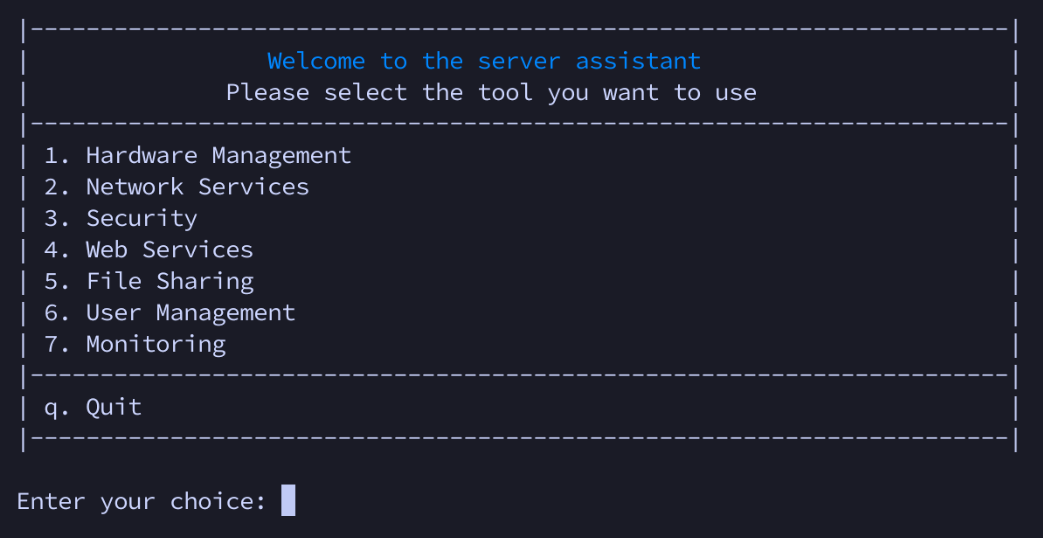
\includegraphics[width=\textwidth]{main.png}
    \caption{Aperçu du script principal \texttt{main.sh} gérant les déploiements automatisés.}
    \label{fig:script-main}
\end{figure}

\begin{figure}[H]
    \centering
    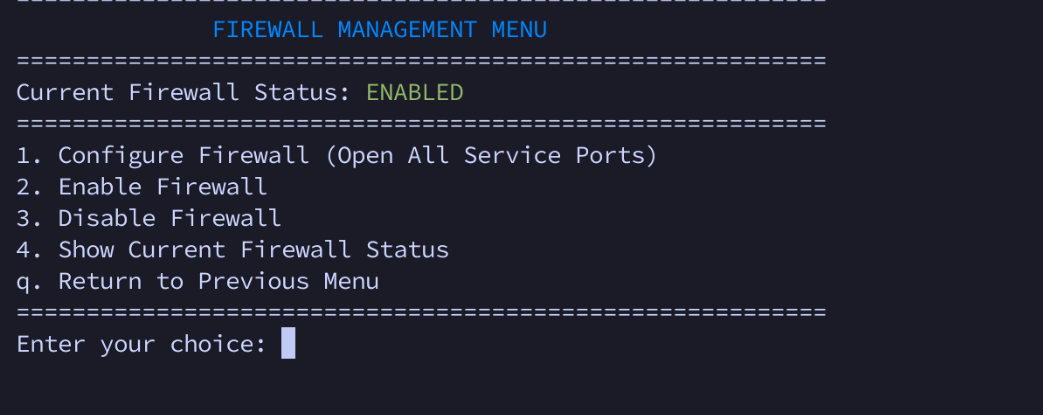
\includegraphics[width=\textwidth]{firewall.png}
    \caption{Aperçu du script \texttt{security.sh} gérant les règles de firewalls.}
    \label{fig:script-firewall}
\end{figure}

\begin{figure}[H]
    \centering
    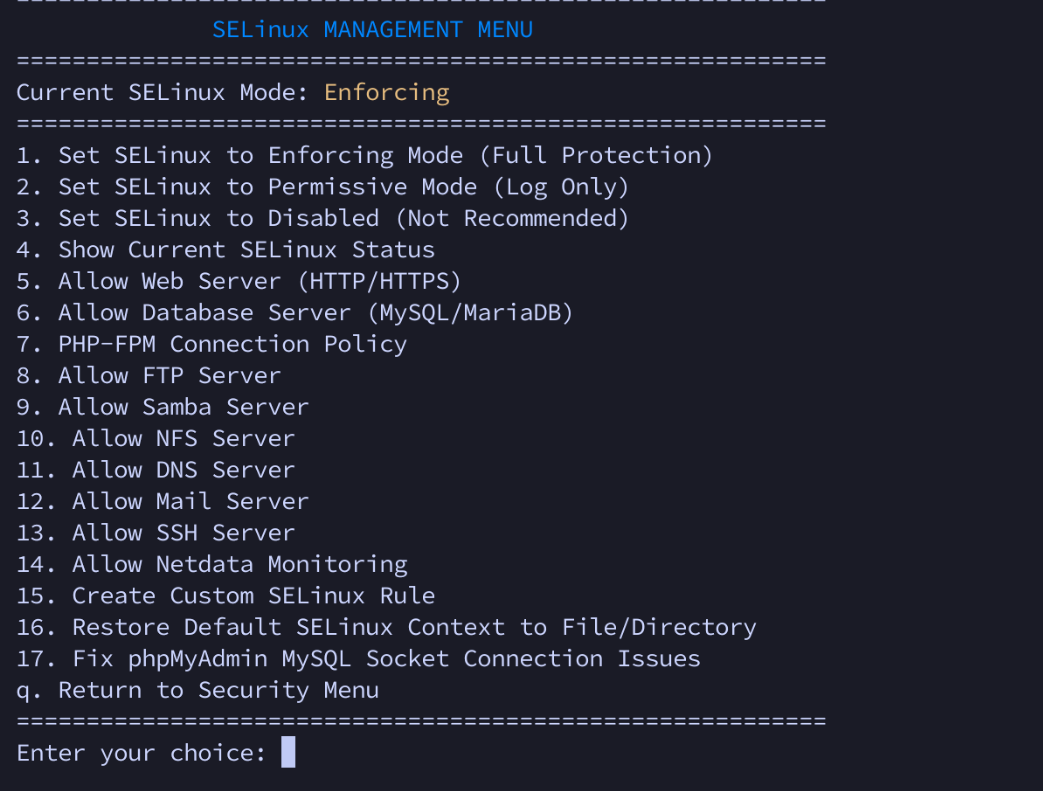
\includegraphics[width=\textwidth]{selinux.png}
    \caption{Aperçu du script \texttt{security.sh} gérant les règles selinux.}
    \label{fig:script-selinux}
\end{figure}

\begin{figure}[H]
    \centering
    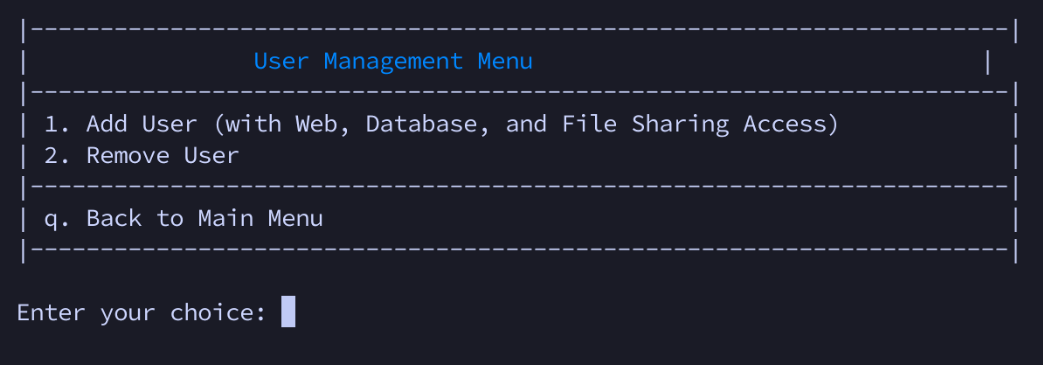
\includegraphics[width=\textwidth]{users.png}
    \caption{Aperçu du script \texttt{usermanagement.sh} gérant les utilisateurs.}
    \label{fig:script-usermanagement}
\end{figure}

\FloatBarrier

Ce programme de script permet la configuration complète de A à Z des différents services et toutes les configurations matérielles et de sécurité du système, facilitant ainsi la gestion et le déploiement.
\newpage
\section{Problèmes rencontrés}

\begin{itemize}
	\item \textbf{Problèmes d'authentification AWS} : difficultés persistantes avec l'authentification à AWS S3 et S3 Glacier malgré l'utilisation des bonnes clés API et secrets pour accéder aux buckets. Malgré plusieurs tentatives avec différentes permissions IAM, les clés d'accès étaient systématiquement refusées, nous obligeant à adopter une solution alternative.
	
	\item \textbf{Instabilité réseau} : qualité médiocre de la connexion rendant la communication extrêmement lente, compliquant significativement les opérations de déploiement et maintenance. Les temps de latence importants ont rendu difficile le débogage en temps réel.
	
	\item \textbf{Dysfonctionnements de l'infrastructure AWS} : gel inexpliqué de plusieurs instances qui ont repris leur fonctionnement plusieurs heures après, sans qu'aucun problème de configuration ne soit détecté (les mêmes scripts de configuration fonctionnant parfaitement sur un serveur Linode). Ces problèmes nous ont contraints à reconfigurer trois instances vierges le jour même de l'évaluation, limitant notre capacité à implémenter des configurations de sécurité encore plus avancées.
\end{itemize}

\section{Conclusion}

Malgré les difficultés techniques rencontrées, ce projet nous a permis d'acquérir des compétences solides en gestion et sécurisation d'infrastructures Linux dans un contexte professionnel. Les solutions mises en oeuvre offrent un compromis équilibré entre sécurité, performance et facilité d'administration.

Nous avons réussi à atteindre les objectifs principaux du projet en déployant une infrastructure complète d'hébergement multi-utilisateur avec :
\begin{itemize}
    \item Une gestion centralisée des utilisateurs, simplifiant l'administration
    \item Des services web sécurisés avec Apache, PHP, PhpMyAdmin et MariaDB
    \item Des solutions de partage de fichiers avec SAMBA, FTP et NFS
    \item Un système de monitoring en temps réel
    \item Des sauvegardes automatisées et fiables
    \item Une sécurité multicouche protégeant contre différentes menaces
\end{itemize}

Si nous avions disposé de davantage de temps, nous aurions pu développer les aspects suivants :
\begin{itemize}
    \item Mise en place d'une solution de haute disponibilité sur plusieurs noeuds
    \item Configuration de sécurité plus avancée (php no exec, options de montages correctes et poussée)
    \item Api entre noeud (pour ajouter un enregistrement dns sur l'instance dédiée au réseau, etc)
    \item Mise en place d'un monitoring plus poussé (ex: déploiement d'un Wazuh pour le monitoring de sécurité)
\end{itemize}

Néanmoins, les fondations sont solides et l'infrastructure répond aux exigences initiales du projet, tout en démontrant notre capacité à adapter notre approche face aux contraintes techniques rencontrées.

\section{Bibliographie}

\begin{thebibliography}{9}
\bibitem{aws} Documentation officielle AWS, \textit{Amazon Web Services Documentation}, \url{https://docs.aws.amazon.com/}

\bibitem{amazonlinux} Documentation Amazon Linux 2023, \textit{Amazon Linux 2023 User Guide}, \url{https://docs.aws.amazon.com/fr_fr/linux/al2023/ug/al2023-ug.pdf}

\bibitem{bind} ISC BIND 9 Documentation, \textit{BIND 9 Administrator Reference Manual}, \url{https://kb.isc.org/docs/aa-01031}

\bibitem{chrony} The Chrony Project, \textit{Chrony Documentation}, \url{https://chrony.tuxfamily.org/documentation.html}

\bibitem{apache} The Apache Software Foundation, \textit{Apache HTTP Server Documentation}, \url{https://httpd.apache.org/docs/}

\bibitem{mariadb} MariaDB Foundation, \textit{MariaDB Server Documentation}, \url{https://mariadb.com/kb/en/documentation/}

\bibitem{samba} Samba Team, \textit{Samba Documentation}, \url{https://www.samba.org/samba/docs/}

\bibitem{vsftpd} Chris Evans, \textit{vsftpd Documentation}, \url{https://security.appspot.com/vsftpd.html}

\bibitem{netdata} Netdata Inc., \textit{Netdata Documentation}, \url{https://learn.netdata.cloud/docs/}

\bibitem{selinux} Red Hat, \textit{SELinux User's and Administrator's Guide}, \url{https://access.redhat.com/documentation/en-us/red_hat_enterprise_linux/7/html/selinux_users_and_administrators_guide/}
\end{thebibliography}

\section{Annexes}

\subsection{Gestion de projet}

\paragraph{Trello}
Pour la gestion des tâches et le suivi des délais du projet, nous avons utilisé un tableau Trello accessible à l'adresse suivante :\\ \url{https://trello.com/invite/b/6823356ebf1cd401ea0175e8/ATTI3a52839bae87ca535511781bc7c023eaEEC1B0DF/projet-linux}

\paragraph{GitHub}
Le code source des scripts sont disponibles dans le dépôt GitHub :\\ \url{https://github.com/sametcatakli/projet-linux-aws}

\end{document}